\documentclass[12pt]{article}

% Packages
\usepackage[utf8]{inputenc}
\usepackage{amsmath}
\usepackage{amssymb}
\usepackage{graphicx}
\usepackage{hyperref}
\usepackage{geometry}
\usepackage{float}

% remove the indent at the beginning of a paragraph:
\setlength{\parindent}{0pt}

% Line spacing
\renewcommand{\baselinestretch}{1}

% distance between new paragraphs:
\setlength{\parskip}{0.5em}

% Title design:
\usepackage{titling}
\pretitle{\begin{center}\LARGE\bfseries}
\posttitle{\par\end{center}\vspace{-0.5em}}
\preauthor{\begin{center}\large}
\postauthor{\par\end{center}\vspace{-2em}}
\predate{\begin{center}\large}
\postdate{\par\end{center}\vspace{-1em}}


% Geometry settings
\geometry{
    a4paper,
    total={170mm,257mm},
    left=20mm,
    right=20mm,
    top=20mm,
    bottom=20mm,
}

% Set the figure counter to reset within subsections
\counterwithin{figure}{subsection}

% Document
\begin{document}

% Title Page
\title{Homework 2: Active Learning + GNNs}
\author{Naomi Derel 325324994, Gili Cohen 326280815, Renana Shachak 213920010}
\date{01.08.2024}
\maketitle

\section{Active Learning}

\subsection{Pipeline Structure}

The pipeline we used for active learning is as follows:
\begin{enumerate}
    \item Load the dataset and split it into the train and test indices provided. Find the features and labels from the given dataset.
    \item For a set number of iterations:
    \begin{itemize}
        \item Train a model on the labeled set.
        \item Use the model to predict the labels of the test set, and calculate an accuracy score.
        \item Select a number of samples from the unlabeled set according to a budget, using one of the selection criterions. Update the labeled set with the new samples and remove said samples from the available pool.
    \end{itemize}
    \item Output the accuracy scores for each iteration. Alternatively, output the final trained model.
\end{enumerate}

\subsection{Uncertainty-Based Selection}

The measure we picked for uncertainty-based selection is entropy. 

The entropy of a distribution is a measure of the uncertainty in that distribution, and so it is a classical measure for our case. 

We calculated the entropy of the output of the model for each sample in the pool, and defined it as an estimate for the uncertainty of the model on said sample. We then selected the samples with the highest entropy to be labeled next, since they are the samples the model is most uncertain about.

\subsection{Custom Selection}

The measure we picked for custom selection is the density selection measure we saw in class.

The density selection is based upon the intuition that the model will benefit the most from samples that extend the vector space the model has seen so far. We used it by calculating the distance of each sample in the pool from the samples the model has seen so far, and then selecting the samples with the lowest density.

For defining the density measure, we tried two approaches (where $x_i$ are the samples the model has seen so far, and $x$ is the sample we are calculating the density for):

\begin{enumerate}
    \item The lowest sum of distances from the samples the model has seen: $ \sum_{i=1}^{n} distance(x_i, x) $.
    \item A density measure based on the sum of exponential distances from the samples the model has seen so far: $ \sum_{i=1}^{n} \exp(-distance(x_i, x)) $.
    This is based on a Gaussian kernel, and is a common measure for density.
\end{enumerate}
The first approach ended up achieving identical or better results, so we used it for the final implementation.

We then selected the samples with the highest density to be labeled next.

Before comparing different parameters, we ran intial trials of the selection criterions with the suggested parameters.

\begin{figure}[H]
    \centering
    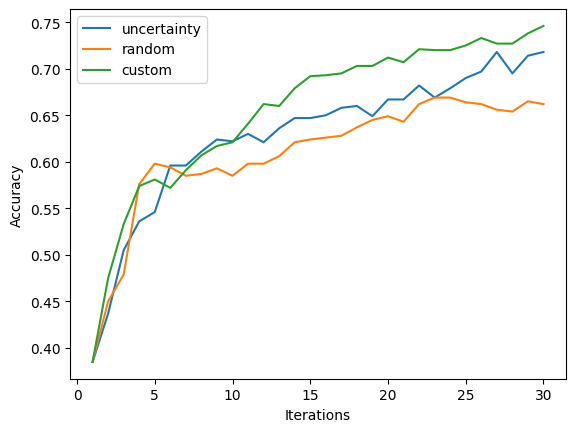
\includegraphics[width=0.8\textwidth]{random_forest_train.png}
    \caption{Comparison of Training Process for Random Forest Model with Different Selection Criteria}
\end{figure}

\subsection{Parameter Comparison}

We compared the results of multiple combinations of models, iterations, and budget per iteration as instructed. We defined pairs of iterations and budget per iteration to be under the limit of 600.

The following tables contain the final accuracy score for each combination. In bold, we present the best results by model, and underlined are the best results overall per selection method.

\subsubsection*{Random Selection}

\begin{table}[H]
    \centering
    \begin{tabular}{|c|c|c|c|}
        \hline
        & SVC & Random Forest & Logistic Regression \\
        \hline
        10 Iterations + 59 Budget & 0.686 & 0.68 & 0.677 \\
        15 Iterations + 39 Budget & 0.68 & \textbf{0.69} & \underline{\textbf{0.707}} \\
        30 Iterations + 19 Budget & \textbf{0.69} & 0.688 & 0.701 \\
        \hline
    \end{tabular}
    \caption{Results of Parameter Comparison for Random Selection}
\end{table}

\subsubsection*{Uncertainty-Based Selection}

\begin{table}[H]
    \centering
    \begin{tabular}{|c|c|c|c|}
        \hline
        & SVC & Random Forest & Logistic Regression \\
        \hline
        10 Iterations + 59 Budget & 0.699 & 0.699 & 0.699 \\
        15 Iterations + 39 Budget & 0.705 & 0.705 & 0.705 \\
        30 Iterations + 19 Budget & \underline{\textbf{0.718}} & \underline{\textbf{0.718}} & \underline{\textbf{0.718}} \\
        \hline
    \end{tabular}
    \caption{Results of Parameter Comparison for Uncertainty-Based Selection}
\end{table}


\subsubsection*{Custom Selection}

\begin{table}[H]
    \centering
    \begin{tabular}{|c|c|c|c|}
        \hline
        & SVC & Random Forest & Logistic Regression \\
        \hline
        10 Iterations + 59 Budget & 0.733 & 0.733 & 0.733 \\
        15 Iterations + 39 Budget & 0.729 & 0.729 & 0.729 \\
        30 Iterations + 19 Budget & \underline{\textbf{0.746}} & \underline{\textbf{0.746}} & \underline{\textbf{0.746}} \\
        \hline
    \end{tabular}
    \caption{Results of Parameter Comparison for Custom Selection}
\end{table}

\subsubsection*{Comparison by Selection}

We now compare the training process for the model which achieved the best results of each selection method. For the selections with tied results, we chose to show the Logistic Regression model for consistency.
Notice that the training process for the random criterion is shorter since the best results were achieved with fewer iterations.

\begin{figure}[H]
    \centering
    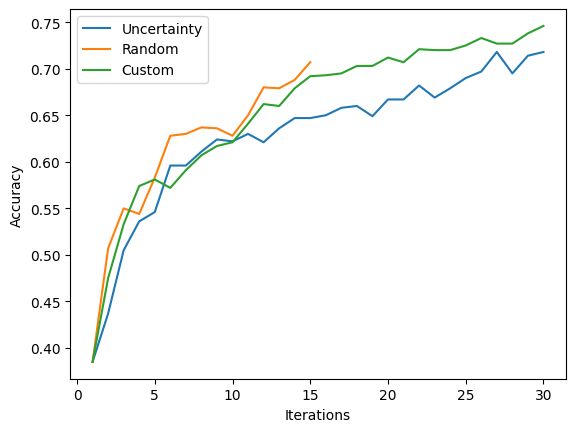
\includegraphics[width=0.8\textwidth]{criterion_comparison.png}
    \caption{Comparison of Training Process for Best Results by Selection Method}
\end{figure}

Overall, we can see the custom criterion with 30 iterations and 19 budget per iteration achieved the best results, with an accuracy score of 0.746 (regardless of the model used).

\subsubsection*{Analysis and Discussion}

The results show a few interesting points. Firstly, when using an advanced selection method (not random), the chosen model does not affect the results but the combination of iterations and budget per iteration does. This might mean that the models are equally good at learning from the data, but the selection method and iterations are key to the success of the active learning process.

Secondly, both the custom and uncertainty criterions achieved the best results with the same combination of iterations and budget per iteration. This might mean that the two methods are similar in their effectiveness, but the custom method is more stable and consistent in its results.

 The random selection model, however, has changes in performance based both on the model used and the combination of iterations and budget. In addition, the results obtained from the random model changed drastically when we ran the code multiple times, while the other methods remained the same as they have no dynamic elements. 


\vspace{1em}
\textsl{Note:} We used the $tqdm$ library to show a progress bar for the iterations, which violates the instruction to not alter the provided code lines. We thought it would be helpful to show the progress of the iterations, while maintaining the original code structure and functionality.

\end{document}